%%
%% This is file `sample-sigchi.tex',
%% generated with the docstrip utility.
%%
%% The original source files were:
%%
%% samples.dtx  (with options: `sigchi')
%% 
%% IMPORTANT NOTICE:
%% 
%% For the copyright see the source file.
%% 
%% Any modified versions of this file must be renamed
%% with new filenames distinct from sample-sigchi.tex.
%% 
%% For distribution of the original source see the terms
%% for copying and modification in the file samples.dtx.
%% 
%% This generated file may be distributed as long as the
%% original source files, as listed above, are part of the
%% same distribution. (The sources need not necessarily be
%% in the same archive or directory.)
%%
%% The first command in your LaTeX source must be the \documentclass command.
\documentclass[sigchi-a]{acmart}

%%
%% \BibTeX command to typeset BibTeX logo in the docs
\AtBeginDocument{%
  \providecommand\BibTeX{{%
    \normalfont B\kern-0.5em{\scshape i\kern-0.25em b}\kern-0.8em\TeX}}}

%% Rights management information.  This information is sent to you
%% when you complete the rights form.  These commands have SAMPLE
%% values in them; it is your responsibility as an author to replace
%% the commands and values with those provided to you when you
%% complete the rights form.
\setcopyright{acmcopyright}
\copyrightyear{2019}
\acmYear{2019}
\acmDOI{10.1145/1122445.1122456}

%% These commands are for a PROCEEDINGS abstract or paper.
\acmConference[Woodstock '18]{Woodstock '18: ACM Symposium on Neural
  Gaze Detection}{June 03--05, 2018}{Woodstock, NY}
\acmBooktitle{Woodstock '18: ACM Symposium on Neural Gaze Detection,
  June 03--05, 2018, Woodstock, NY}
\acmPrice{15.00}
\acmISBN{978-1-4503-9999-9/18/06}


%%
%% Submission ID.
%% Use this when submitting an article to a sponsored event. You'll
%% receive a unique submission ID from the organizers
%% of the event, and this ID should be used as the parameter to this command.
%%\acmSubmissionID{123-A56-BU3}

%%
%% The majority of ACM publications use numbered citations and
%% references.  The command \citestyle{authoryear} switches to the
%% "author year" style.
%%
%% If you are preparing content for an event
%% sponsored by ACM SIGGRAPH, you must use the "author year" style of
%% citations and references.
%% Uncommenting
%% the next command will enable that style.
%%\citestyle{acmauthoryear}

%%
%% end of the preamble, start of the body of the document source.
\begin{document}

%%
%% The "title" command has an optional parameter,
%% allowing the author to define a "short title" to be used in page headers.
\title{HiveTracker: 3D Positioning for Ubiquitous Embedded Systems}

%%
%% The "author" command and its associated commands are used to define
%% the authors and their affiliations.
%% Of note is the shared affiliation of the first two authors, and the
%% "authornote" and "authornotemark" commands
%% used to denote shared contribution to the research.
\author{C\'edric Honnet}
%\orcid{1234-5678-9012}
\affiliation{%
  \institution{Sorbonne University}
  \department{UPMC, CNRS, ISIR}
  \streetaddress{}
  \city{Paris}
  \country{France}}
\email{cedric@honnet.eu}

\author{Gon\c{c}alo Lopes}
\affiliation{%
  \institution{NeuroGEARS Ltd}
  \streetaddress{}
  \city{London}
  \country{United Kingdom}}
\email{g.lopes@neurogears.org}


%%
%% By default, the full list of authors will be used in the page
%% headers. Often, this list is too long, and will overlap
%% other information printed in the page headers. This command allows
%% the author to define a more concise list
%% of authors' names for this purpose.
%\renewcommand{\shortauthors}{Honnet and Lopes}

%%
%% The abstract is a short summary of the work to be presented in the
%% article.
\begin{abstract}
  Recent advances in positional tracking systems for virtual and augmented reality have opened up the possibility for ubiquitous motion capture technology in the consumer market. However, for many applications in performance art, athletics, neuroscience, and medicine, these systems remain too bulky and expensive for general use, and can track only a few objects at a time. In this work, we present the new cross-platform WebBLE interface and real-time in-browser visualization for the HiveTracker, a small wireless device that takes advantage of existing lighthouse tracking technology to provide affordable, scalable, and highly accurate positional tracking capabilities. We show how the new developments will reduce the setup costs and increase the broader accessibility of our tracking technology.
\end{abstract}

%%
%% The code below is generated by the tool at http://dl.acm.org/ccs.cfm.
%% Please copy and paste the code instead of the example below.
%%

\begin{CCSXML}
<ccs2012>
<concept>
<concept_id>10003120.10003121.10003125</concept_id>
<concept_desc>Human-centered computing~Interaction devices</concept_desc>
<concept_significance>500</concept_significance>
</concept>
</ccs2012>
\end{CCSXML}

\ccsdesc[500]{Human-centered computing~Interaction devices}


%%
%% Keywords. The author(s) should pick words that accurately describe
%% the work being presented. Separate the keywords with commas.
\keywords{open-source, low cost, motion capture, wireless device, virtual reality, tracker}


%%
%% This command processes the author and affiliation and title
%% information and builds the first part of the formatted document.
\maketitle

\section{Introduction}
Robust real-time positional tracking systems have been the target of research for decades to support applications in natural user interfaces (NUI), virtual reality (VR) and augmented reality (AR). All of these interface paradigms require an accurate sampling of the spatial environment of a user, and have to be responsive in real-time in order to sustain the illusion of control. Recent developments in motion sensing and tracking technology for VR have finally moved the field of motion capture technology away from expensive custom engineered spaces with multiple cameras. The need to deploy VR at scale in the consumer market has pushed for scalable and cost-effective solutions, mostly through inside-out techniques using either computer vision based simultaneous localization and mapping (SLAM) or laser-based lighthouse approaches.

Because each device is taking care of its own localization, such inside-out solutions are inherently scalable, allowing for a much larger number of devices to coexist in the same space. This has triggered many researchers to start rethinking the entire approach to full-body motion tracking, replacing the passive reflective beads with active inside-out devices. Unfortunately, size and accuracy remain a limitation for such motion capture applications. Inside-out SLAM based computer vision devices rely on cameras and expensive processors, which both make existing controllers more bulky and increase power requirements.

An alternative solution to inside-out tracking is to use a beacon-based approach, such as the one used in the Valve Lighthouse tracking system. In this system, a lighthouse base station periodically sweeps the space with a laser at a fixed frequency. Photodiodes placed in tracked objects can detect these sweeps and using either information embedded in modulated light at the beam, or synchronization pulses, can reconstruct the exact angle at which the laser hit the object. Positioning information can be accurately recovered from the photodiodes as long as the timing of each laser hit can be sensed fast enough.

In previous work, we explored the design of a PCB prototype called the HiveTracker \cite{Quinones2018}, that takes advantage of dedicated real-time sensing capabilities of the Nordic nRF52 microcontroller to sense the lighthouse light sweeps without requiring a dedicated FPGA. This allowed us to design an embedded device with up to five photodiodes that is small, accurate, and cheap enough for full-body motion tracking at scale.

In this paper, we describe the further development of our prototype, and the main hardware and software challenges we had to overcome to increase the accessibility and ease of use of the HiveTracker beyond a proof-of-concept research prototype.

\section{Contributions}

\begin{itemize}
  \item {\itshape Open-source firmware supporting} low-latency serial BLE communication protocol for any number of devices.
  \item {\itshape BLE interface for 3D reconstruction and triangulation} of positional data from each device.
  \item {\itshape Real-time JavaScript visualization} of reconstructed positioning data for rapid-prototyping and testing.
\end{itemize}

\section{Firmware}

\begin{marginfigure}
  \centering
  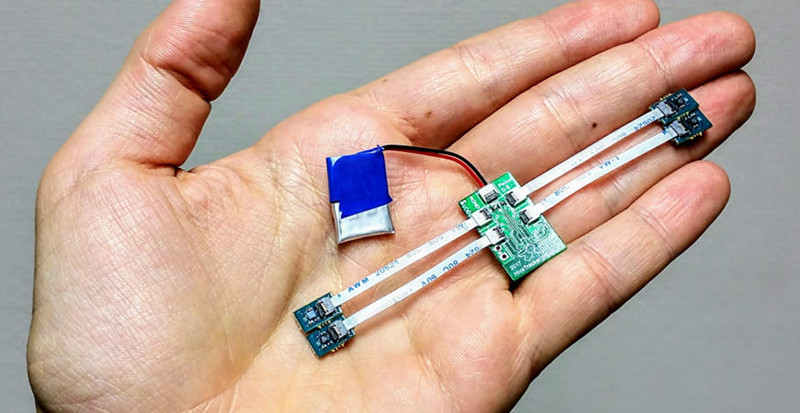
\includegraphics[width=\linewidth]{prototype}
  \caption{1907 Franklin Model D roadster. Photograph by Harris \&
    Ewing, Inc. [Public domain], via Wikimedia
    Commons. (\url{https://goo.gl/VLCRBB}).}
  \Description{The 1907 Franklin Model D roadster.}
\end{marginfigure}

\section{BLE interface}

\section{Real-time visualization}

\section{Future work}

\section{Related work}

\section{SIGCHI Extended Abstracts}

The ``\verb|sigchi-a|'' template style (available only in \LaTeX\ and
not in Word) produces a landscape-orientation formatted article, with
a wide left margin. Three environments are available for use with the
``\verb|sigchi-a|'' template style, and produce formatted output in
the margin:
\begin{itemize}
\item {\verb|sidebar|}:  Place formatted text in the margin.
\item {\verb|marginfigure|}: Place a figure in the margin.
\item {\verb|margintable|}: Place a table in the margin.
\end{itemize}

%%
%% The acknowledgments section is defined using the "acks" environment
%% (and NOT an unnumbered section). This ensures the proper
%% identification of the section in the article metadata, and the
%% consistent spelling of the heading.
\begin{acks}
The authors would like to thank Julien Mellet for early work on reconstruction and fusion algorithms, and NeuroGEARS Ltd for the financial support and all the help that they provide. This project was also partially funded by the "Human Computer Interface Prize" from the Hack-A-Day organization. Finally, this work was also partially performed within the Labex SMART (ANR-11-LABX-65), supported by French state funds managed by the ANR under reference ANR-11-IDEX-0004-02.
\end{acks}

%%
%% The next two lines define the bibliography style to be used, and
%% the bibliography file.
\bibliographystyle{ACM-Reference-Format}
\bibliography{ubicomp-2019}

%%
%% If your work has an appendix, this is the place to put it.
%\appendix

\end{document}
\endinput
%%
%% End of file `sample-sigchi.tex'.
